\section{Results}\label{sec:results}

\begin{table*}[t]
\centering
\small
\caption{Development results for the three 640-recording seed pairs. The selected update identifies the clean-BCE checkpoint. Stressed counts use repeated views.}\label{tab:development}
\begin{tabular}{@{}lrrrrrr@{}}
\toprule
Seed and arm & Update & Clean AUC & Stress AUC & Stress FA & Stress miss & B clean FA \\
\colrule
9107 ERM & 560 & 0.9872 & 0.6715 & 54/336 & 222/336 & 19/144 \\
9107 CHANNEL & 760 & 0.9814 & 0.8026 & 45/336 & 155/336 & 31/144 \\
9207 ERM & 520 & 0.9851 & 0.5946 & 167/336 & 143/336 & 26/144 \\
9207 CHANNEL & 720 & 0.9809 & 0.7839 & 70/336 & 134/336 & 20/144 \\
9307 ERM & 360 & 0.9822 & 0.5498 & 44/336 & 266/336 & 21/144 \\
9307 CHANNEL & 680 & 0.9856 & 0.7934 & 61/336 & 119/336 & 30/144 \\
\botrule
\end{tabular}
\end{table*}


\begin{table*}[t]
\centering
\small
\setlength{\tabcolsep}{3pt}
\caption{Channel minus ERM. Brackets give within-seed 95 percent speaker-cluster intervals. Mean and sample SD describe the three fitted contrasts. Error differences are percentage points.}\label{tab:uncertainty}
\begin{tabular}{@{}lrrrr@{}}
\toprule
Endpoint & 9107 & 9207 & 9307 & Mean and SD \\
\colrule
A macro stress AUC & \shortstack[r]{+0.1312\\{[+0.0207, +0.2387]}} & \shortstack[r]{+0.1893\\{[+0.0932, +0.2684]}} & \shortstack[r]{+0.2436\\{[+0.1884, +0.3071]}} & +0.1880 $\pm$ 0.0562 \\
A clean REAL FA & \shortstack[r]{+0.00\\{[-2.68, +2.68]}} & \shortstack[r]{+0.00\\{[-2.68, +2.68]}} & \shortstack[r]{+1.79\\{[-3.57, +9.82]}} & +0.60 $\pm$ 1.03 \\
A clean FAKE miss & \shortstack[r]{+2.68\\{[+0.00, +6.25]}} & \shortstack[r]{+0.00\\{[-3.57, +4.46]}} & \shortstack[r]{-1.79\\{[-4.46, +1.79]}} & +0.30 $\pm$ 2.25 \\
A stress REAL FA & \shortstack[r]{-2.68\\{[-8.63, +4.76]}} & \shortstack[r]{-28.87\\{[-37.20, -19.05]}} & \shortstack[r]{+5.06\\{[-1.79, +10.42]}} & -8.83 $\pm$ 17.78 \\
A stress FAKE miss & \shortstack[r]{-19.94\\{[-25.31, -14.58]}} & \shortstack[r]{-2.68\\{[-10.42, +3.57]}} & \shortstack[r]{-43.75\\{[-47.92, -39.58]}} & -22.12 $\pm$ 20.62 \\
B clean REAL FA & \shortstack[r]{+8.33\\{[+1.39, +17.36]}} & \shortstack[r]{-4.17\\{[-6.94, -0.69]}} & \shortstack[r]{+6.25\\{[-1.39, +15.28]}} & +3.47 $\pm$ 6.70 \\
A05 stress FAKE miss & \shortstack[r]{+3.70\\{[-3.70, +12.70]}} & \shortstack[r]{+16.67\\{[+3.70, +29.82]}} & \shortstack[r]{-11.11\\{[-16.67, -5.26]}} & +3.09 $\pm$ 13.90 \\
A06 stress FAKE miss & \shortstack[r]{+7.41\\{[-6.67, +22.92]}} & \shortstack[r]{+27.78\\{[+11.76, +43.75]}} & \shortstack[r]{-31.48\\{[-43.86, -17.54]}} & +1.23 $\pm$ 30.11 \\
\botrule
\end{tabular}
\end{table*}


\subsection{Overall Robustness with Channel Augmentation}

Table~\ref{tab:development} summarizes the six 640-record development curves. Macro stress ROC-AUC increases by 0.1312, 0.1893 and 0.2436 for 9107, 9207 and 9307, respectively. The mean and sample SD across seeds are 0.6053 \ensuremath{\pm} 0.0616 for ERM, 0.7933 \ensuremath{\pm} 0.0094 for channel, and +0.1880 \ensuremath{\pm} 0.0562 for their paired difference. The clean AUC difference is negative in the first two seeds and positive in 9307. Figure~\ref{fig:aggregate} links the two arms within each seed.

Clean A REAL false alarms tie in the first two pairs and increase from 4 to 6 of 112 in 9307. Clean A FAKE misses increase from 6 to 9 in 9107, tie at 9 in 9207, and decrease from 10 to 8 in 9307. Clean B REAL false alarms increase in 9107 and 9307 and decrease in 9207. Table~\ref{tab:uncertainty} separates within-seed speaker intervals from descriptive variation across fitted pairs.

All three 640-recording development A macro stress AUC intervals exclude zero. In 9307 the paired interval is [0.1884, 0.3071]. The 9207 stress miss interval includes zero. These intervals quantify speaker resampling conditional on each fitted pair and shared development protocol.

In the nested seed-9207 comparison, the channel-minus-ERM macro stress AUC gain decreases from +0.1893 at 640 recordings to +0.1081 at 1,280 (Table~\ref{tab:size-sensitivity}). Equation~\eqref{eq:size-contrast} gives a difference of \ensuremath{-}0.0812, with a pointwise 95\% paired speaker interval of [\ensuremath{-}0.1421, \ensuremath{-}0.0148]. Both fitted pairs gain in ranking. The gain is smaller under the larger fixed-epoch protocol, which also uses twice as many optimizer updates.

\begin{table*}[t]
\caption{Development A by condition. Each cell gives ROC-AUC / REAL false alarms / FAKE misses. Each error count has 112 sources of its class.}\label{tab:conditions}
\centering
\begin{tabular}{@{}lrrrr@{}}
\toprule
Condition & 9107 ERM & 9107 Channel & 9207 ERM & 9207 Channel \\
\colrule
Clean & 0.9872 / 3 / 6 & 0.9814 / 3 / 9 & 0.9851 / 4 / 9 & 0.9809 / 4 / 9 \\
Half gain & 0.9812 / 0 / 15 & 0.9818 / 0 / 14 & 0.9758 / 0 / 16 & 0.9820 / 0 / 15 \\
Quarter gain & 0.9237 / 7 / 20 & 0.9576 / 0 / 17 & 0.9278 / 9 / 20 & 0.9590 / 0 / 19 \\
Noise5 & 0.6567 / 1 / 99 & 0.7793 / 8 / 64 & 0.5449 / 22 / 77 & 0.7579 / 13 / 56 \\
Opus64 & 0.9884 / 6 / 4 & 0.9819 / 4 / 6 & 0.9861 / 9 / 5 & 0.9839 / 5 / 8 \\
Noise to Opus & 0.6763 / 48 / 38 & 0.8108 / 28 / 37 & 0.6408 / 104 / 13 & 0.7981 / 44 / 26 \\
Opus to Noise & 0.6814 / 5 / 85 & 0.8178 / 9 / 54 & 0.5981 / 41 / 53 & 0.7958 / 13 / 52 \\
\botrule
\end{tabular}
\end{table*}


\begin{figure*}[t]
\centering
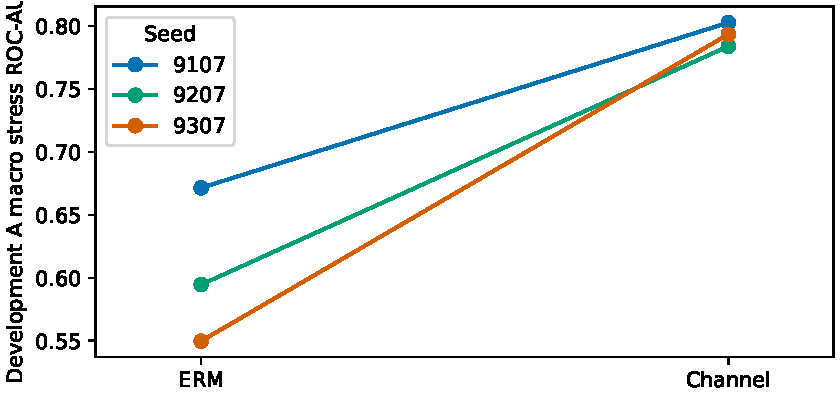
\includegraphics[width=.89\textwidth]{aggregate_v5.pdf}
\caption{Development macro stress ROC-AUC for the three initialization blocks. Lines connect the two arms within a seed.}\label{fig:aggregate}
\end{figure*}

The locked evaluation completed 17,408 predictions for the original four selected models. Table~\ref{tab:heldout-endpoints} reports aggregate results and Table~\ref{tab:heldout-conditions} separates the conditions. Macro stressed ROC-AUC increased in both seed blocks, from 0.8308 to 0.8875 in 9107 and from 0.7498 to 0.8948 in 9207. The corresponding paired speaker-cluster intervals for channel minus ERM were [0.0296, 0.0842] and [0.1158, 0.1752]. These positive differences were smaller than the development A contrasts. Figure~\ref{fig:heldout-contrasts} compares the predefined endpoints across partitions. Figure~\ref{fig:heldout-roc} shows the score-level ranking under each held-out condition.

Stressed FAKE misses fell from 1,370 to 587 in 9107 and from 815 to 453 in 9207, each out of 2,496 views from 832 FAKE sources. The rate differences were \ensuremath{-}31.37 points [\ensuremath{-}33.41, \ensuremath{-}29.36] and \ensuremath{-}14.50 points [\ensuremath{-}17.38, \ensuremath{-}11.67]. Stressed REAL false alarms increased by one in 9107, from 80/768 to 81/768 (+0.13 points), and fell from 322/768 to 136/768 in 9207. The 768 views in each comparison came from 256 REAL sources. The paired intervals were [\ensuremath{-}3.23, +3.76] and [\ensuremath{-}29.07, \ensuremath{-}19.03] percentage points. All endpoint and attack intervals used 10,000 valid draws.

\begin{table*}[t]
\centering
\small
\caption{Fixed-epoch training-size sensitivity for seed 9207 on the same development sources. Column headings give the training size. A has 112 sources per class and B has 144 REAL sources. Pooled stress counts use three views per source at threshold 0.5. Each attack row uses 18 sources.}\label{tab:size-sensitivity}
\begin{tabular}{@{}lrrrr@{}}
\toprule
Development endpoint & ERM 640 & Channel 640 & ERM 1,280 & Channel 1,280 \\
\colrule
A clean ROC-AUC & 0.9851 & 0.9809 & 0.9900 & 0.9860 \\
A macro stress ROC-AUC & 0.5946 & 0.7839 & 0.7062 & 0.8143 \\
A clean REAL false alarms & 4/112 & 4/112 & 1/112 & 3/112 \\
A clean FAKE misses & 9/112 & 9/112 & 3/112 & 8/112 \\
A stress REAL false alarms & 167/336 & 70/336 & 5/336 & 161/336 \\
A stress FAKE misses & 143/336 & 134/336 & 248/336 & 64/336 \\
B clean REAL false alarms & 26/144 & 20/144 & 18/144 & 22/144 \\
A05 stressed FAKE misses & 38/54 & 47/54 & 50/54 & 36/54 \\
A06 stressed FAKE misses & 16/54 & 31/54 & 50/54 & 11/54 \\
\botrule
\end{tabular}
\end{table*}


\begin{figure*}[t]
\centering
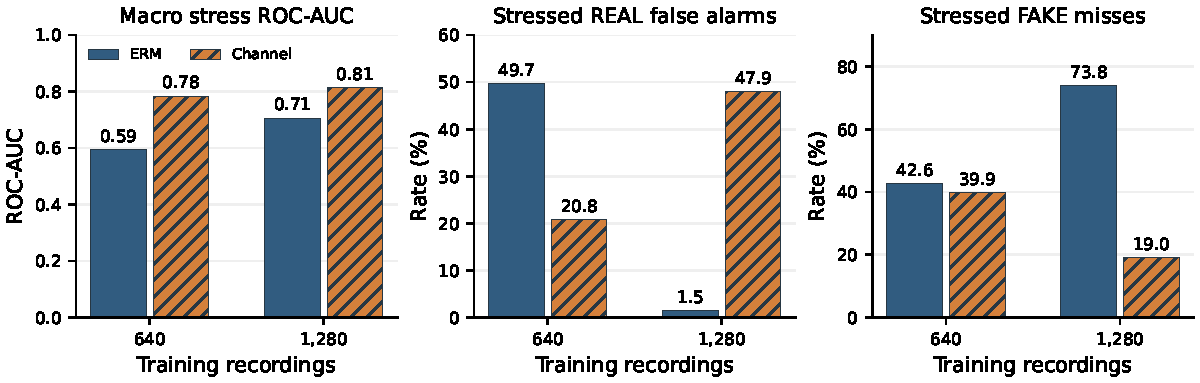
\includegraphics[width=.97\textwidth]{size_sensitivity_v7.pdf}
\caption{Seed-9207 development A results on the same recordings at both training sizes. Macro stress ROC-AUC averages three condition-level AUCs. Each pooled error rate uses 336 views from 112 sources of its class at threshold 0.5. Bars show observed values. Table~\ref{tab:size-sensitivity} gives counts and the text reports the paired intervals.}\label{fig:size-sensitivity}
\end{figure*}

\subsection{Class-Asymmetric Errors and Operating-Point Trade-offs}

With 1,280 samples, Channel improves stressed FAKE misses from 248 to 64 out of 336 (\ensuremath{-}54.76 points) and increases stressed REAL false alarms from 5 to 161 out of 336 (+46.43 points). With 640 samples, the respective contrast for REAL false alarms is \ensuremath{-}28.87 points, leading to a size contrast of +75.30 points (pointwise 95\% speaker interval [62.50, 87.80]). Figure~\ref{fig:size-sensitivity} illustrates that better ranking is accompanied by switching the class of errors at the threshold 0.5.

The selected 1,280 Channel checkpoint violates both registered +2-point clean-risk guards. Development A clean FAKE misses rose from 3/112 to 8/112 (+4.46 points) and B clean REAL false alarms rose from 18/144 to 22/144 (+2.78 points). Pointwise 95\% speaker intervals were [1.79, 6.25] and [\ensuremath{-}4.86, 11.81] percentage points. The B interval includes zero. The guards use the observed differences for the pair selected by clean BCE, so both exceed the tolerance.

Table~\ref{tab:conditions} breaks down the parts of the macro stress outcome. The table and ROC figure detail the first two seeds. The channel arm also increases AUC under all registered stress conditions in 9307. Figure~\ref{fig:roc} depicts the complete ROC curves associated with these AUCs. Fixed-threshold changes remain heterogeneous. Under Noise5, FAKE misses fall from 99 to 64 in 9107 and from 77 to 56 in 9207. The corresponding REAL false-alarm counts rise from 1 to 8 in 9107 and fall from 22 to 13 in 9207.

\begin{table*}[t]
\caption{Selected-model results on the locked held-out subset. Stress error counts pool three views per source. Macro stress ROC-AUC averages the three condition-specific AUCs.}\label{tab:heldout-endpoints}
\centering
\small
\begin{tabular}{@{}lrrrr@{}}
\toprule
Endpoint & 9107 ERM & 9107 Channel & 9207 ERM & 9207 Channel \\
\colrule
Macro stress ROC-AUC & 0.8308 & 0.8875 & 0.7498 & 0.8948 \\
Stress FAKE miss & 1370/2496 & 587/2496 & 815/2496 & 453/2496 \\
Stress REAL false alarm & 80/768 & 81/768 & 322/768 & 136/768 \\
Clean REAL false alarm & 25/256 & 19/256 & 22/256 & 16/256 \\
Clean FAKE miss & 125/832 & 129/832 & 127/832 & 147/832 \\
\botrule
\end{tabular}
\end{table*}


\begin{table*}[t]
\caption{Condition-specific held-out performance. Each cell gives ROC-AUC / REAL false alarms / FAKE misses. There are 256 REAL and 832 FAKE recordings per condition.}\label{tab:heldout-conditions}
\centering
\small
\begin{tabular}{@{}lrrrr@{}}
\toprule
Condition & 9107 ERM & 9107 Channel & 9207 ERM & 9207 Channel \\
\colrule
Clean & 0.9534 / 25 / 125 & 0.9436 / 19 / 129 & 0.9507 / 22 / 127 & 0.9410 / 16 / 147 \\
Noise5 & 0.8053 / 0 / 701 & 0.8655 / 12 / 259 & 0.6815 / 28 / 492 & 0.8765 / 25 / 193 \\
Noise to Opus & 0.8447 / 76 / 143 & 0.8991 / 53 / 143 & 0.8196 / 226 / 38 & 0.9044 / 89 / 93 \\
Opus to noise & 0.8424 / 4 / 526 & 0.8979 / 16 / 185 & 0.7483 / 68 / 285 & 0.9034 / 22 / 167 \\
\botrule
\end{tabular}
\end{table*}


The larger 9207 REAL benefit under the two compositions is visible in the per-condition counts. Noise-to-Opus false alarms fall from 104 to 44, while its FAKE misses increase from 13 to 26. By way of contrast, REAL false alarms go from 41 down to 13, while FAKE misses go from 53 down to 52. Both counts have denominator 112. The starting point with the high number of REAL false alarms for the condition of Noise-to-Opus allows a sizable decrease in this operating point. It would not be accurate to refer to the decrease itself as an advantage across classes.

For the stress results, gain controls and Opus64 for the two development seeds give some perspective. For quarter gain, the channel arm has fewer false alarms and higher AUC in both blocks. For standalone Opus64, the channel arm has fewer false alarms but higher FAKE misses in both blocks. The control of 64 kb/s uses a different rate from the compositions of 24 kb/s. It is listed as a separate condition, and any comparison against the chains would alter the codec and noise conditions as well. The 24 kb/s control is the correct one for standalone comparison against 9107 and 9207.

In 9307, stress FAKE misses fall from 266 to 119 of 336 while REAL false alarms rise from 44 to 61 of 336. This contrasts with fewer stressed REAL false alarms in 9107 and 9207. The 9307 stress miss contrast is \ensuremath{-}43.75 percentage points (95\% speaker interval [\ensuremath{-}47.92, \ensuremath{-}39.58]). The contrast for its stress REAL false alarm is +5.06 points (interval [\ensuremath{-}1.79, +10.42]). B clean false alarms increase from 21 to 30 out of 144, which is a change of +6.25 points (95\% speaker interval [\ensuremath{-}1.39, +15.28]). The difference is greater than the registered +2-point guard for the selected CLEAN\_BCE pair. The interval represents speaker resampling in the pair and does not affect the observed guard choice.

In 9207, decreases in other attack instances balance 24 extra A05 and A06 missed instances under stress conditions. The A05 and A06 attacks add six extra missed instances in 9107. The differences include transformed views. Table~\ref{tab:attackconditions} gives the number of A05 and A06 attacks that get an additional correct or missed decision in at least one stress condition. Figure~\ref{fig:transitions} provides the paired analysis for both classes under A.

\begin{figure*}[t]
\centering
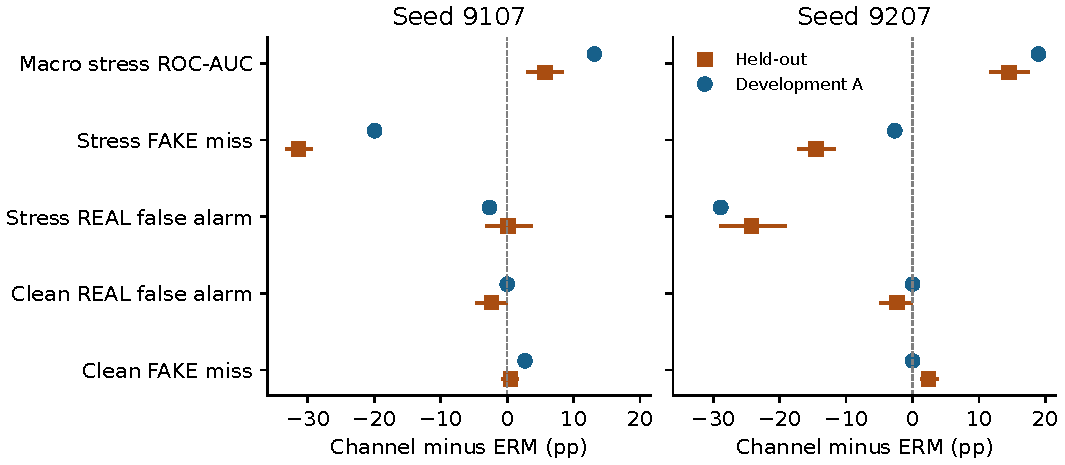
\includegraphics[width=.94\textwidth]{heldout_contrasts.pdf}
\caption{Channel-minus-ERM contrasts on development A and the locked held-out subset, separately by seed. Held-out segments show 95\% paired speaker-cluster percentile intervals. AUC differences are multiplied by 100. Positive differences indicate better AUC or higher error rates. Cohorts and attack populations differ across partitions.}\label{fig:heldout-contrasts}
\end{figure*}

Clean REAL false alarms fell from 25 to 19 in 9107 and from 22 to 16 in 9207, out of 256 sources per arm. Clean FAKE misses increased from 125 to 129 and from 127 to 147 out of 832, while clean ROC-AUC declined from 0.9534 to 0.9436 and from 0.9507 to 0.9410. The 9207 clean FAKE miss increase was 2.40 percentage points [1.15, 3.86]. Development B showed opposite false-alarm directions between the two seeds. The cohorts differ in speaker and source support.

The sums for stress reflect the existence of the operating point shift. For Noise5, the misses of FAKE dropped from 701 to 259 and from 492 to 193 out of 832. With respect to Opus and then Noise10, the misses of FAKE dropped from 526 to 185 and from 285 to 167. In case of the reverse sequence, Noise10 followed by Opus, the misses of FAKE remained constant at 143 in 9107 and increased from 38 to 93 in 9207, while the number of REAL false alarms decreased from 226 to 89 out of 256 and AUC increased from 0.8196 to 0.9044.

Post hoc analysis shows that at the threshold of 0.5 the operating point has shifted. When Noise10 and then Opus were applied in 9207, the two algorithms agreed on 85 real false alarms, channel corrected 141 and made four. In case of FAKE, they agreed on 20 misses, channel corrected 18 and introduced 73. In 9107, when the two algorithms were subjected to Noise10 and then Opus, the sum of 143 FAKE misses included 93 shared misses, 50 corrected and 50 introduced. The numbers reflect decision-making on the same sources.

In Fig.~\ref{fig:v4-operating}, the retro-grid ensures that the registered threshold remains at 0.5. On held-out 9207 under Noise10 followed by Opus24, channel augmentation gives fewer false alarms and more misses at every sampled threshold from 0.20 through 0.80. The miss direction reverses at 0.10 and 0.90. For Noise5 and the opposite order, FAKE misses decrease at all 11 sampled thresholds in both seeds, with condition- and seed-dependent REAL errors. FAKE misses cleaned in 9207 rise for all thresholds sampled. These comparisons describe the measured score grid and provide no threshold-selection rule.

Score distributions also change locally around the registered boundary. Under Noise10 followed by Opus24 in 9207, 7 versus 30 of 256 REAL scores and 5 versus 18 of 832 FAKE scores lie within 0.025 of 0.5 for ERM and channel, respectively. The supplement gives the confusion matrices for every arm and condition, empirical curve coordinates and the 0.025 and 0.05 score windows. Development B supplies only REAL scores. Its FNR, ROC-AUC and EER are undefined.

\begin{figure*}[t]
\centering
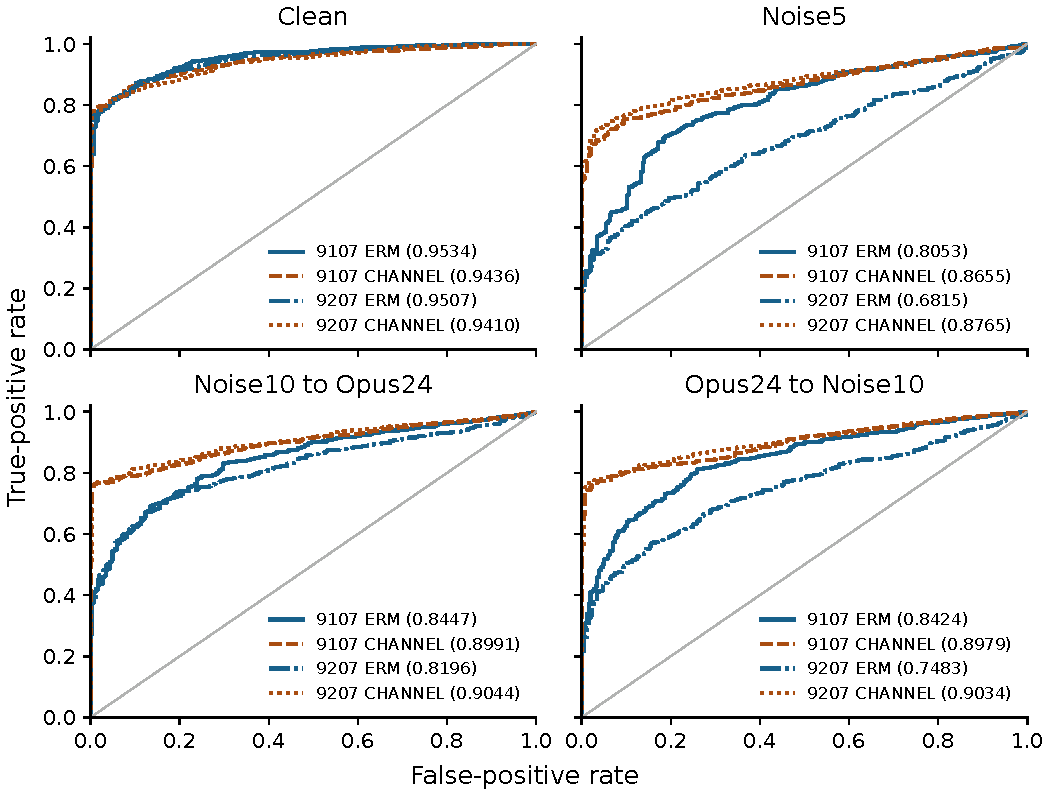
\includegraphics[width=.86\textwidth]{heldout_roc.pdf}
\caption{Empirical held-out ROC curves for four selected models. Each panel contains 256 REAL and 832 FAKE recordings, evaluated under the named condition. Legends give seed, method, and AUC. The same sources recur across conditions.}\label{fig:heldout-roc}
\end{figure*}

\subsection{Attack-Specific Robustness and Failure Modes}

For seed 9207, the A05 contrast changes from 38/54 versus 47/54 at 640 to 50/54 versus 36/54 at 1,280 (ERM versus Channel). A06 changes from 16/54 versus 31/54 to 50/54 versus 11/54. Each denominator represents three correlated stress views from 18 sources. Both training size and update budget changed. Seed 9307 compares initializations at 640. Table~\ref{tab:attack} and Fig.~\ref{fig:attack} show both sign reversals. Channel increases A05 and A06 stress misses in the first two pairs and decreases them in 9307. The latter changes are \ensuremath{-}6/54 and \ensuremath{-}17/54, respectively. The pointwise 9307 speaker intervals are [\ensuremath{-}16.67, \ensuremath{-}5.26] and [\ensuremath{-}43.86, \ensuremath{-}17.54] percentage points, respectively. The 9107 intervals include zero. These within-seed intervals do not establish a stable attack effect across initializations.

Table~\ref{tab:attackconditions} details the first two seeds. In 9307, all six A05 recoveries occur in the noise-before-Opus condition. For A06, 18 recoveries and one new miss occur across the three stress views. Net recoveries span five A05 speakers and six A06 speakers. The A06 ERM burden is 16 of 54 in 9207 and 45 of 54 in 9307. Differences in baseline burden and FAKE score crossings describe where the reversal occurs. They leave the underlying model or generator mechanism unresolved.

\begin{figure*}[t]
\centering
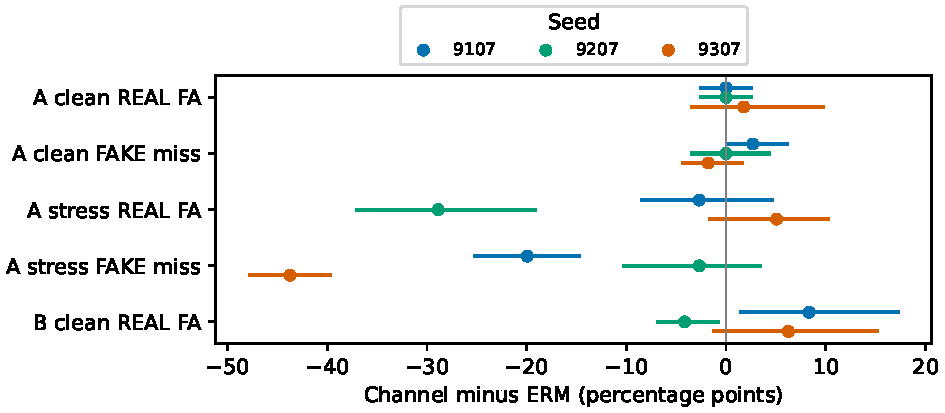
\includegraphics[width=.91\textwidth]{classwise_errors_v5.pdf}
\caption{Channel-minus-ERM fixed-threshold error rates by development stratum, class, and seed. Segments show within-seed paired speaker-cluster percentile intervals. REAL errors are false alarms and FAKE errors are misses. Clean A has 112 recordings per class, stress A has 336 views from 112 recordings per class, and clean B has 144 REAL recordings.}\label{fig:classwise}
\end{figure*}

\begin{table*}[t]
\centering
\small
\caption{Development A05/A06 stress FAKE misses over the three stress views. Each row represents 18 distinct sources and 54 transformed views.}\label{tab:attack}
\begin{tabular}{@{}lrrr@{}}
\toprule
Seed and attack & ERM & Channel & $\Delta$ misses \\
\colrule
9107 A05 & 48/54 & 50/54 & +2 \\
9107 A06 & 41/54 & 45/54 & +4 \\
9207 A05 & 38/54 & 47/54 & +9 \\
9207 A06 & 16/54 & 31/54 & +15 \\
9307 A05 & 49/54 & 43/54 & -6 \\
9307 A06 & 45/54 & 28/54 & -17 \\
\botrule
\end{tabular}
\end{table*}


Figure~\ref{fig:speakers} shows that two B speakers contribute 10 of the 12 net additional false alarms in 9107. For 9207, reductions occur across several speakers. B contains only REAL recordings, and the counts are interpreted as false alarms with no B ROC-AUC or EER.

Figure~\ref{fig:heldout-attacks} shows the condition-specific FAKE miss contrasts. Pooled stressed misses fell on A07--A16 and rose on A17--A19 in both blocks. A17, A18 and A19 added 10, 11 and 4 misses in 9107 and 43, 43 and 56 in 9207, each out of 192 views from 64 sources per attack. The pointwise 9107 intervals include zero. The 9207 intervals exclude zero: [15.90, 29.03], [14.12, 30.81] and [20.63, 37.70] percentage points. The development A05/A06 results concern a separate attack set.

In the post-hoc grouping, A07--A16 account for 808 and 504 fewer stressed misses in 9107 and 9207, partly offset by 25 and 142 additional misses on A17--A19. For A17--A19, Noise-to-Opus added 39 misses in 9107. All three stress conditions added misses in 9207. On A19, 43/64 sources acquired a miss in at least one stress condition and 18/64 in multiple conditions. These exploratory groupings were identified after reviewing held-out results. The pointwise intervals have no multiplicity adjustment.

\begin{figure*}[t]
\centering
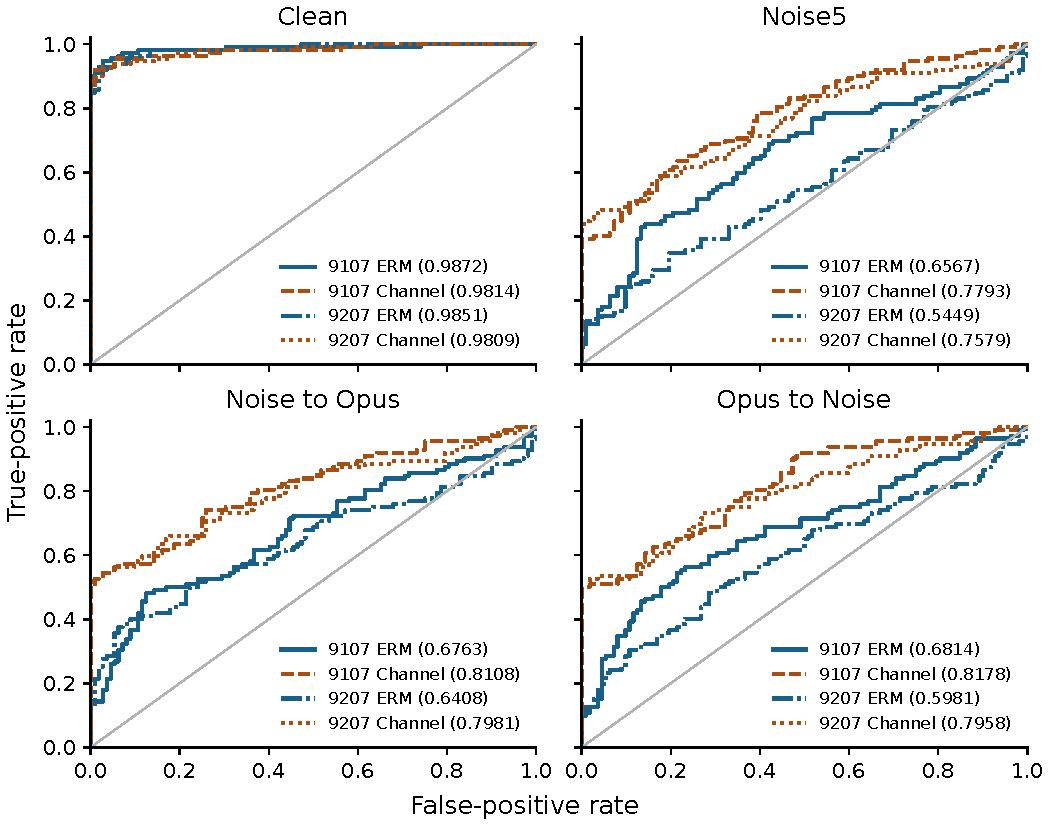
\includegraphics[width=.88\textwidth]{development_roc.pdf}
\caption{Empirical ROC curves from the four selected models in the first two seeds on development A. Each panel ranks the same 112 REAL and 112 FAKE recordings under one condition. Legends give the seed, method, and recomputed AUC. The diagonal denotes chance ranking.}\label{fig:roc}
\end{figure*}

\subsection{Transformation-Order Effects}

For the same 112 A REAL recordings at seed 9207, the Channel-minus-ERM contrast in the signed order error gap (Noise-to-Opus minus Opus-to-Noise) changes from \ensuremath{-}28.57 points at 640 to +26.79 points at 1,280. The size contrast is +55.36 points (pointwise 95\% speaker interval [32.12, 79.46]). The change in the corresponding signed FAKE-score difference is \ensuremath{-}0.2099 to +0.0764. These paired contrasts measure detector response to the order of processing. See the supplement for the counts exclusive and inclusive to each arm and class. In the first two development blocks, out of 112 A REAL sources, the Noise-to-Opus-only false-alarm counts change from 43 to 19 in 9107 and 63 to 31 in 9207. The opposite order has no exclusive REAL false alarms in A. Among 112 A FAKE sources, Opus-to-Noise alone causes 48 versus 17 misses in 9107 and 40 versus 26 in 9207. The Noise-to-Opus-only FAKE counts are 1 versus 0 and 0 versus 0. In the 9307 pair, there is also the same order asymmetry classwise. Noise-to-Opus-only REAL errors have shifted from 37 to 44, while Opus-to-Noise-only FAKE errors have shifted from 41 to 33, both in a sample of 112. The signed FAKE score gap decreases from 0.2375 to 0.0538 in the median. Figure~\ref{fig:order} represents paired score differences before the thresholding point.

9107 retrospective diagnostics produce 1,472 predicted values for Noise10 and Opus24 separately. Matched waveforms help recover not only registered sequences but also selected anchor values that were replayed without drifting. A leave-one-speaker-out nuisance regression yields directional class-discrimination AUCs of 0.538 for ERM and 0.432 for channel on the signed order score. This measures a residual score contrast on the development cohort. The same standalone components were evaluated for seed 9207 on all 368 development sources, adding 1,472 predictions. All 18 clean and ordered score anchors matched their sealed values exactly. On development A, standalone Noise10 FAKE misses decreased from 82 to 54 in 9107 and changed from 47 to 48 in 9207, out of 112 per arm. Under standalone Opus24, 9207 REAL false alarms decreased from 19 to five and FAKE misses increased from two to ten. The 9107 nuisance regression remains a single-seed analysis. These component results constrain interpretation of the compositions and do not identify a forensic mechanism.

\begin{figure*}[t]
\centering
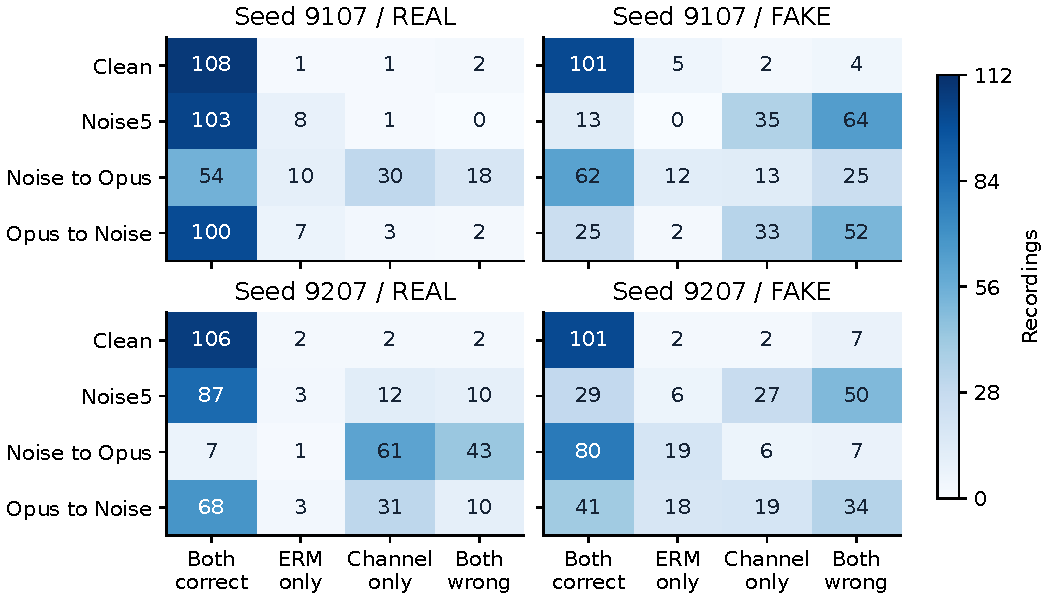
\includegraphics[width=.96\textwidth]{source_transitions.pdf}
\caption{Within-source correctness for the first two seeds at threshold 0.5 on development A. Each row contains 112 recordings of the indicated class. The same recordings contribute to each condition row. The two middle columns identify sources correctly classified by only one method.}\label{fig:transitions}
\end{figure*}

\begin{table*}[t]
\caption{A05 and A06 source-level diagnostics. Each condition has 18 sources. Error cells are ERM / channel. Harm and recovery can overlap across views.}\label{tab:attackconditions}
\centering
\small
\begin{tabular}{@{}lrrrrrr@{}}
\toprule
Seed / attack & Clean & Noise5 & Noise to codec & Codec to noise & All stress & Harmed / rec. \\
\colrule
9107 / A05 & 0 / 0 & 17 / 17 & 14 / 16 & 17 / 17 & 14 / 16 & 3 / 1 \\
9107 / A06 & 3 / 6 & 18 / 16 & 7 / 12 & 16 / 17 & 6 / 12 & 7 / 2 \\
9207 / A05 & 0 / 0 & 17 / 17 & 7 / 13 & 14 / 17 & 7 / 13 & 8 / 0 \\
9207 / A06 & 5 / 7 & 9 / 12 & 0 / 5 & 7 / 14 & 0 / 5 & 10 / 0 \\
\botrule
\end{tabular}
\end{table*}


Source-linked order asymmetry persisted. In 9107, REAL sources wrong only under noise-to-Opus numbered 72 for ERM and 37 for channel, with zero exclusive errors in the reverse direction. In 9207 the corresponding counts were 158 and 68, while exclusive reverse-order errors numbered zero and one. Among FAKE sources, reverse-order-only misses numbered 384 and 43 in 9107 and 247 and 74 in 9207. The opposite exclusive FAKE miss counts were one and one in 9107, and zero and zero in 9207. Each model uses the same 256 REAL and 832 FAKE sources in the order comparison.

\begin{figure*}[t]
\centering
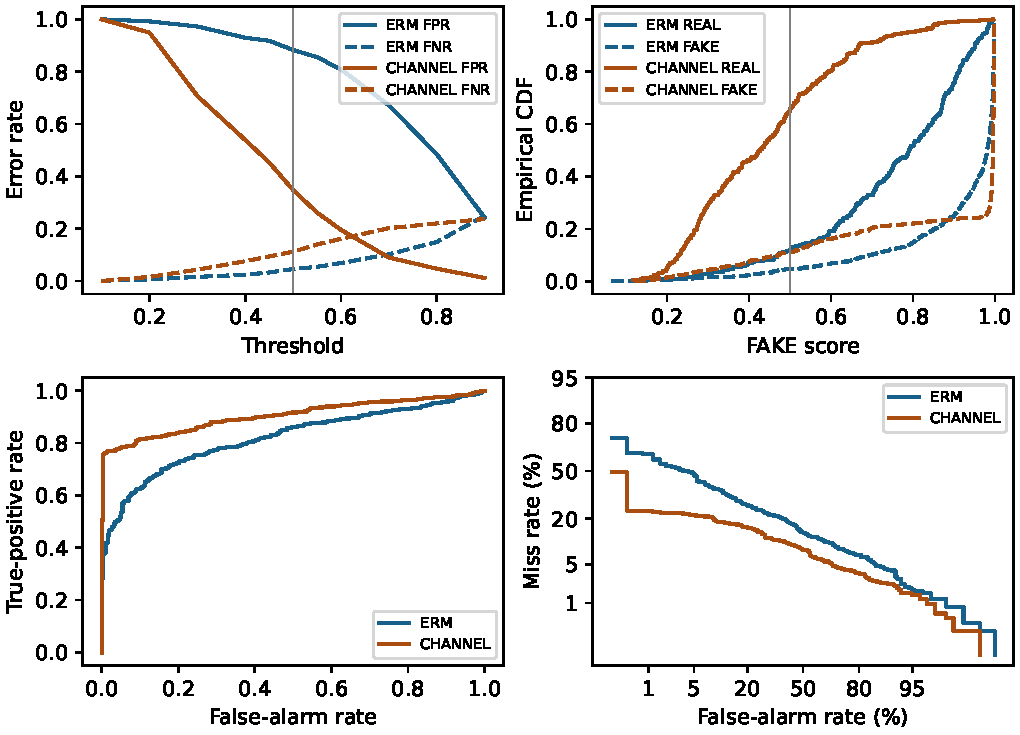
\includegraphics[width=.95\textwidth]{operating_points_v4.pdf}
\caption{Held-out seed 9207 under Noise10 followed by Opus24. Top left shows exploratory FPR and FNR at 11 thresholds. Top right shows class-specific empirical CDFs. Bottom panels show empirical ROC and DET. DET axes use a normal quantile transform and clip endpoint rates at half an event per class. The vertical lines identify the registered threshold of 0.5. Each arm has 256 REAL and 832 FAKE sources.}\label{fig:v4-operating}
\end{figure*}

The score contrasts shown in Fig.~\ref{fig:heldout-order} were also directional, with reduced median FAKE scores following channel adaptation. The median score contrasts in FAKE became 0.3454 and 0.0063 in 9107, 0.2419 and 0.0076 in 9207. However, small score contrasts cannot automatically be assumed to reflect a superior decision rule, in view of the fact that attack-specific misses occurred. Speaker-related scores exhibit the same order error pattern distribution. In the case of ERM 9107, the reverse-minus-forward FAKE error contrast was 16 out of 21 FAKE recordings for speaker LA\_0045 and 13 out of 21 for speaker LA\_0046.

\subsection{Robustness, Stability and Generalization}

The direction of the development stress ranking gain and FAKE miss reduction is consistent across all three pairs. The magnitude of the gain, as well as the direction of false-alarm results, varies according to the selected pair. Common development data allow for a comparison of initializations using the protocol described above, in which case speaker uncertainty is computed in each pair separately.

The fixed epoch size experiment includes a development-only comparison for seed 9207. The three initializations correspond to 640 recordings. The held-out evaluation evaluates the original 640 recording model corresponding to seeds 9107 and 9207 using additional ASVspoof 2019 LA speakers. Cross-corpus robustness remains untested.

\begin{figure*}[t]
\centering
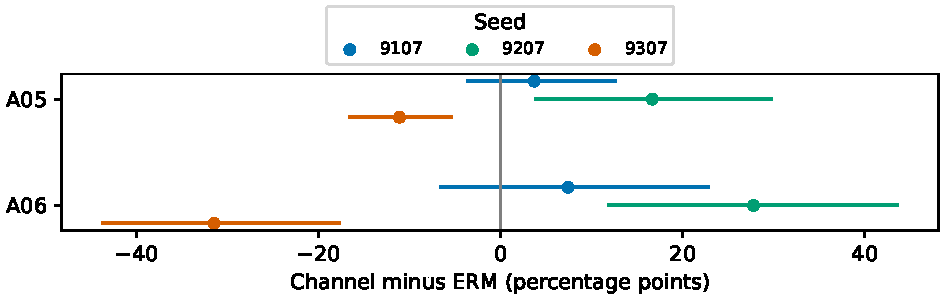
\includegraphics[width=.79\textwidth]{attack_changes_v5.pdf}
\caption{Development A05/A06 stressed FAKE miss changes by seed. Positive values indicate more misses. Intervals resample speakers within a seed. Each attack contributes 54 views from 18 recordings.}\label{fig:attack}
\end{figure*}

\begin{figure*}[t]
\centering
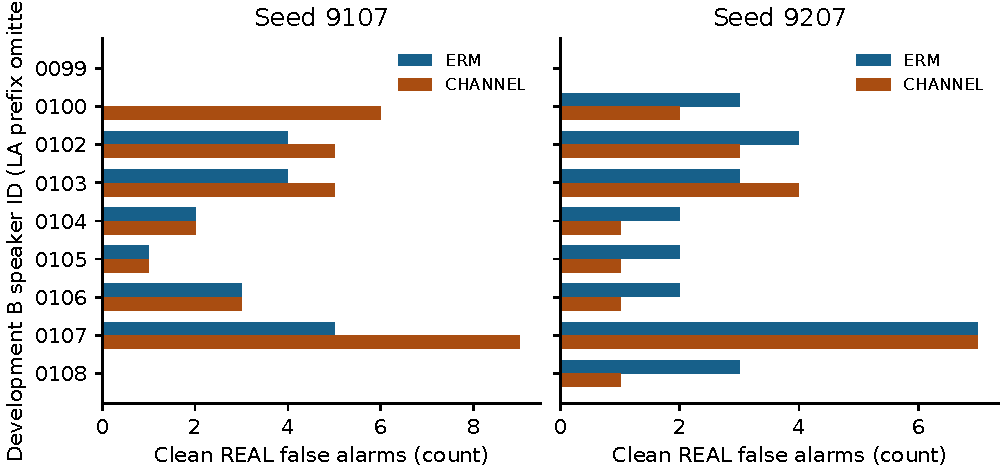
\includegraphics[width=.89\textwidth]{speaker_counts.pdf}
\caption{Clean REAL false alarms by speaker on development B for the first two seeds. Each of nine speakers contributes 16 recordings, for 144 recordings per arm and seed.}\label{fig:speakers}
\end{figure*}

\subsection{Practical Implications and Limitations}

In 9307 the recorded optimizer durations were 39.9 minutes for ERM and 78.9 minutes for channel. At 1,280, the seed-9207 optimizer durations were 78.6 and 160.3 minutes, respectively, with validation taking 37.6 and 37.9 minutes. These are local CPU workload measurements. The architecture and parameter count are shared across training sizes.

A bounded inference benchmark used the clean inputs of the first 12 registered development sources, repeated three times after anchor replay, at batch size one on a single CPU thread. Input duration was capped at 3 s. Median preprocessing time was 10.9 ms (interquartile range 10.3--11.2 ms), forward time 91.3 ms (90.5-93.5 ms), and end-to-end time 102.1 ms (101.1-104.2 ms). The timed preprocessing includes decoding, resampling and the P0 input transform on clean input. The separate headroom and channel-transform stages are outside the timed path. The two 9207 exports each contain 1,308,401 parameters, of which 369,281 are updated during warm-up and 646,481 during partial fine-tuning. The exported stage has 661,920 nontrainable parameters. Each export occupies 5,916,699 bytes. Loading time in one process was 3.35 and 2.81 s, where the second loading came after the first loading. The maximum process working set during the timing process was about 475 MiB. The development convenience sample supports an architectural and local runtime description. Mobile, streaming and concurrent performance remain unmeasured.

\begin{figure*}[t]
\centering
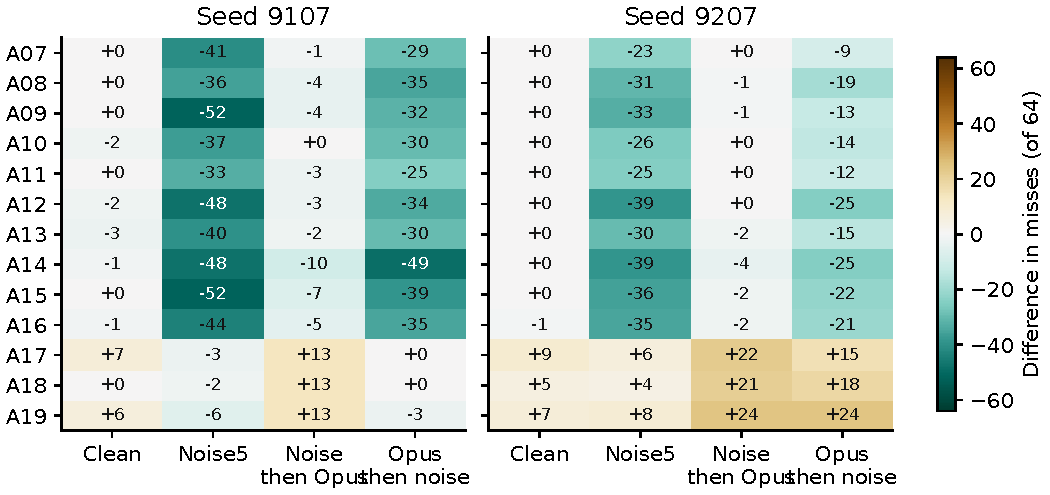
\includegraphics[width=.92\textwidth]{heldout_attacks.pdf}
\caption{Held-out channel-minus-ERM FAKE miss counts by attack, condition and seed. Each cell compares the same 64 sources. Positive counts indicate deterioration and negative counts indicate fewer misses. The full numerical supplement retains both arm counts and stressed attack intervals.}\label{fig:heldout-attacks}
\end{figure*}

The error curves illustrate why a new operating point requires independent validation with costs and traffic prevalence appropriate to the deployment. The ordered chains make it more imperative to validate the position where noise is added vis-a-vis codec operations.
